% -*- TeX-master: "main"; fill-column: 72 -*-

\newcommand{\fixttspace}{\hspace*{1pt}}

\section{Package syntax and semantics}

In this section, we define the syntax and semantics of the Qualitative Models package for SBML Level~3 Version~1.  We expound on the
various data types and constructs defined in this package, then in
\sect{examples}, we provide complete examples of using the constructs in
example SBML models.

\subsection{Namespace URI and other declarations necessary for using this package}
\label{xml-namespace}

Every SBML Level~3 package is identified uniquely by an XML namespace
URI.  For an SBML document to be able to use a given SBML Level~3
package, it must declare the use of that package by referencing its URI.
The following is the namespace URI for this version of the Qualitative Models package for SBML Level~3 Version~1:
\begin{center}
\uri{http://www.sbml.org/sbml/level3/version1/qual/version1}
\end{center}

In addition, SBML documents using a given package must indicate whether
understanding the package is required for complete mathematical
interpretation of a model, or whether the package is optional.  This is
done using the attribute \token{required} on the \token{<sbml>} element
in the SBML document.  For the Qualitative Models package,
the value of this attribute must be set to \val{true}.

The following fragment illustrates the beginning of a typical SBML model
using SBML Level~3 Version~1 and this version of the Qualitative Models package:

\begin{example}
<?xml version="1.0" encoding="UTF-8"?>
<sbml xmlns="http://www.sbml.org/sbml/level3/version1/core" level="3" version="1"
      xmlns:qual="http://www.sbml.org/sbml/level3/version1/qual/version1" qual:required="true">
\end{example}
    

% -----------------------------------------------------------------------------
\subsection{Primitive data types}
\label{primitive-types}

Section~3.1 of the SBML Level~3 specification defines a number of
primitive data types and also uses a number of XML Schema 1.0 data
types \citep{biron:2000}.  We assume and use some of them in the rest of
this specification, specifically \primtype{boolean}, \primtype{ID},
\primtype{SId}, \primtype{SIdRef}, and \primtype{string}. The Qualitative Model package defines other primitive types;
they are described below.

% removed for now
%\subsubsection{Type \fixttspace\primtypeNC{temporisationType}}
%\label{primtype-temporisation}
%
%The \primtype{temporisationType} is an enumeration of values used to indicate the updating policy used by %a \Transition.  The possible values are \const{timer}, \const{priority}, \const{sustain}, \const{proportion} %and \const{rate}.
%
\subsubsection{Type \fixttspace\primtypeNC{sign}}
\label{primtype-sign}

The \primtype{sign} is an enumeration of values used to indicate direction of an \Input within the system.  The possible values are \const{positive}, \const{negative}, \const{dual} and \const{unknown}. 

\subsubsection{Type \fixttspace\primtypeNC{transitionInputEffect}}
\label{primtype-inputeffect}
The \primtype{transitionInputEffect} is an enumeration of values used to indicate the effect of an \Input \Transition within the system.  The possible values are \const{none} and \const{consumption}.

\subsubsection{Type \fixttspace\primtypeNC{transitionOutputEffect}}
\label{primtype-outputeffect}
The \primtype{transitionOutputEffect} is an enumeration of values used to indicate the effect of an \Output \Transition within the system.  The possible values are \const{production} and \const{assignmentLevel}.

\pagebreak
% -----------------------------------------------------------------------------
\subsection{Qualitative modelling}
\label{qual}

Before describing the classes and their attributes that have been used by this Qualitative Models Specification it is worth clarifying the intended meaning of some of the terms used. 

\subsubsection{Levels}

%\TODO{need to address the issue of still allowing symbols in a simple form}

The entities being modelled have a \emph{level} associated with them that indicates the current state of the entity. A \emph{level} is an integer and takes values that range from \val{0} up to and including a maximum.

In future versions of the Qualitative Modelling specification, it is intended to introduce a means of specifying symbols to represent any value that might be appropriate in the model (see ~\sec{apdx:apdx-future}).

%A \emph{symbol} is intended to represent any value that might be appropriate in the model.  A user can %merely define the set of symbols that might be used and how the \token{symbolValue} associated with an %entity might be altered  by the model. 
\smallskip

\subsubsection{Transitions}

Qualitative Models consider \emph{transitions} that alter the levels of entities involved in the model, depending on the level of some other entities.  This may involve the level of an entity being increased or decreased by a fixed amount; the level remaining unchanged; or the level being reassigned to an alternate value. Transitions occur when a set of conditions is met. These conditions may involve the levels falling above or below  a given \emph{threshold}. 

A simple example of this is the case where there are two entities A and B and the model states that when the level of A exceeds \val{1} (the threshold), the level of B is increased by \val{1}. 

\subsubsection{FunctionTerms}

The resulting value of an entity affected by a transition may have several possibilities that are governed by a number of conditions. Each transition can have a list of conditional functions \emph{functionTerms}, each associated with a result that allow the user to specify sets of piecewise conditions. For example a model may wish to encode the following
\smallskip
\begin{center}
$B = \left\{ \begin{array}{ll}
      B+1 & \mbox{if $A < 1$} \\
      B & \mbox{if $1 <= A < 3$} \\
     B + 2 & \mbox{otherwise}  \\
     \end{array}
\right.
$
\end{center}

\smallskip
In this case the \Transition would have a \FunctionTerm for each of the first two conditions and a \DefaultTerm for the otherwise component.


\subsubsection{Interpretation of time}


Transitions occur when a set of conditions are met.  This specification assumes that these conditions are not dependent on time and can occur at any arbitary time point.  Thus the use of any math that explicitly involves time (e.g. the \token{csymbol} \textbf{time} or \textbf{delay}) is not recommended. It is anticipated that future versions will consider time issues see \sec{apdx:apdx-future}.



\subsubsection{Hybrid models}


It is noted in \sec{apdx:apdx-future} that this specification does not facilitate the use of SBML constructs outside the scope of this package within a particular model.  This is an aspect of modelling that will be addresses in future versions.







% -----------------------------------------------------------------------------
\subsection{The extended \class{Model} class}
\label{model-class}

The extension of SBML Level~3 Core's \Model class is relatively
straightforward: the Qualitative Models Package adds two lists,
one for holding qualitativeSpecies (\token{listOfQualitativeSpecies}, of class
\ListOfQualitativeSpecies), and the other for holding transitions (\token{listOfTransitions},
of class \ListOfTransitions).  \fig{qual-extended-model-uml} provides the UML
diagram.  

\pagebreak

The \sbml{Model} element may contain at most one \ListOfQualitativeSpecies, which must contain at least one \QualitativeSpecies. It may also contain at most one \ListOfTransitions which must contain at least one \Transition.The \QualitativeSpecies class and
the \Transition  class are defined in \sect{qualSpecies-class} and \sect{transitions-class} respectively.

\begin{figure}[h!]
  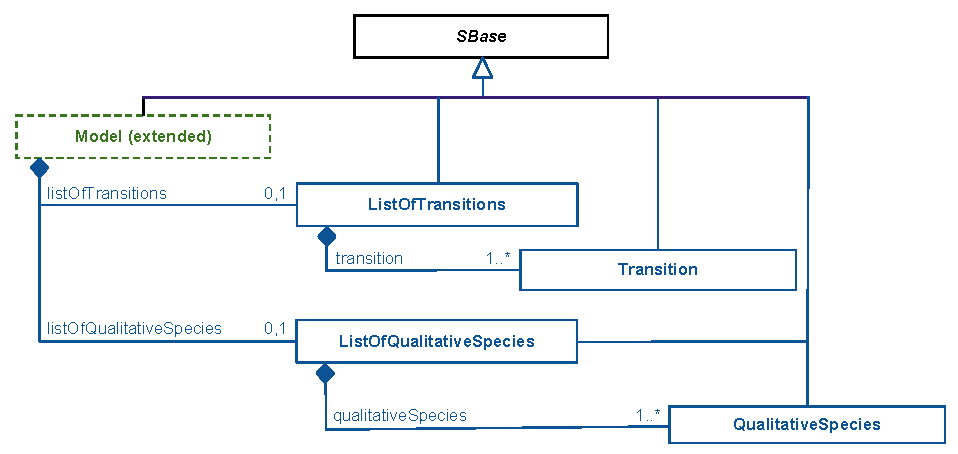
\includegraphics{figs/qual-extended-model-uml.pdf}
  \caption{The definitions of the extended \Model class. In other respects, \Model remains defined as
    in the SBML Level~3 Core specification.}
  \label{qual-extended-model-uml}
\end{figure}


% -----------------------------------------------------------------------------
\subsection{The \class{QualitativeSpecies} class}
\label{qualSpecies-class}
Similarly to the \sbml{Species} in SBML, the components of qualitative models refer to pools of entities that are considered indistinguishable and are each located in a specific \sbml{Compartment}. However, here components are characterised by their qualitative influences rather than by taking part in reactions. Therefore, we define the \QualitativeSpecies element to represent such pools of entities.

In a Petri net, {\em qualitative species} refer to the places of the model, while in a logical model, they refer to the variables of this model (i.e. nodes of the influence graph).

A \QualitativeSpecies describes a pool of indistinguishable entities in a \sbml{Compartment}. It is associated with  a \token{level} (an integer representing e.g. an activity state, or a functional level of concentration, etc.)  %or a \token{symbolValue} from its \ListOfSymbolicValues.
 The \QualitativeSpecies class is defined in \fig{qual-qualitative-species-uml}.
%\TODO{add listOfSymbols back}
\begin{figure}[h]
  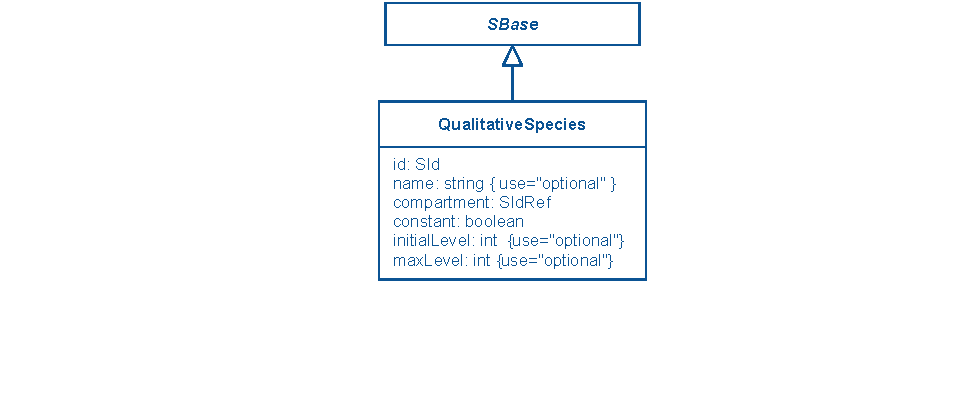
\includegraphics{figs/qual-qualitative-species-uml.pdf}
  \caption{The definitions of the \QualitativeSpecies class. }
  \label{qual-qualitative-species-uml}
\end{figure}

\paragraph{The \fixttspace\token{id} attribute}

The \token{id} attribute takes a required value
of type \primtype{SId}. The \token{id} is used as an identifier for the particular \QualitativeSpecies. It can be used as a 
<ci> element within math elements included by elements defined within the namespace of the Qualitative Models specification i.e. the \token{math} element of a \FunctionTerm, in which case it it interpreted as the \emph{level} of this \QualitativeSpecies. Note that for SBML Level~3 Version~1 identifiers from a given package cannot be referenced by elements outside that package. 

\paragraph{The \fixttspace\token{name} attribute}

A \QualitativeSpecies also has an optional \token{name} attribute of type \primtype{string}. 
 The \token{name} attribute should be used
in the same manner as on SBML Level~3 Core
objects; see Section~3.3.2 of the SBML Level~3 Version~1 Core
specification for more information.


\paragraph{The \token{compartment} attribute}
The required attribute \token{compartment}, of type \primtype{SIdRef}, is used to identify the compartment in which the qualitativeSpecies is located.  The attribute's value must be the identifier of an existing \sbml{Compartment} object in the model.  This attribute is comparable with the \token{compartment} attribute on the \sbml{Species} element.

\paragraph{The \token{constant} attribute}
The required attribute \token{constant}, of type \primtype{boolean}, is used to indicate that the \token{level} of the qualitativeSpecies is fixed or can be varied. This attribute is comparable with the \token{constant} attribute on the \sbml{Species} element.

Typically, in a regulatory or influence graph a \QualitativeSpecies may receive no interaction and if so, would appear only as an \Input in the model and have the value of the \token{constant} attribute set to \val{true}. In other influence graphs or in Petri net models a \QualitativeSpecies may occur as an \Input whose level is changed by the \Transition and would have \token{constant} set to \val{false}.  The nature of changes to a \QualitativeSpecies resulting from a \Transition is also recorded using the \token{transitionEffect} attribute on the \Input (see section \ref{input-class}) and may be set to \val{none} to indicate there is no change. This duplication of information provides a means of validating the modeller's intent and also allows entities on the borders of a system to be easily identified.
 


\paragraph{The \token{initialLevel}  attribute}
The \token{initialLevel} is a non-negative \primtype{integer} that defines the initial \emph{level} of the \QualitativeSpecies in its \sbml{Compartment}. This attribute is optional but cannot exceed the value of the \token{maxlevel} attribute, if both are set.

\paragraph{The \token{maxLevel} attribute}
The \token{maxLevel} is a non-negative \primtype{integer} that sets the maximal \emph{level} of the \qualt{QualitativeSpecies}. This attribute is optional but when set, the \emph{level} of the \QualitativeSpecies must not exceed this value at any point in a simulation.

In logical models, the \token{maxLevel} must be coherent with the \token{resultLevel} values in the function terms defined for the corresponding transition, i.e. the model must not contain a \FunctionTerm that attempts to set a \emph{level} that exceeds this value.

In Petri nets, this attribute is meant to define place capacities. Hence, a transition is not enabled if the value resulting from its firing would exceed the  \token{maxLevel} of one of its output places.  The attribute is not required and even if explicitly stated, the restriction imposed by place capacities in a Petri net model  \textbf{must} be encapsulated within the \token{math} element of the \FunctionTerm elements. 

This attribute can also be used to indicate the range of possible levels for a \QualitativeSpecies whose \token{constant} attribute is true. This may seem a little contradictory, since if the \token{constant} attribute is true then the level associated with the \QualitativeSpecies cannot vary. However, it provides additional information regarding the possible levels particularly in the case where no \token{initialLevel} has been set.

%\subsubsection{The \class{SymbolicValue} class}
%The \QualitativeSpecies element may contain at most one \ListOfSymbolicValues that contains zero or more %\SymbolicValue elements. An empty list is allowed, and useful for e.g. adding annotations.
%
%The \SymbolicValue element defines a non instantiated parameter that allows the model to associate %undefined values with a particular \QualitativeSpecies.
%Symbols can be considered as uninstantiated parameters. Such symbols may represent the different %solutions of piecewise linear differential equations, along with different thresholds.
%
%\paragraph{The \token{id} attribute}
%A \SymbolicValue element has an \token{id} attribute that takes a required value
%of type \primtype{SId}. The \token{id} is used as an identifier for the particluar \SymbolicValue and may be %referenced by the \token{symbolicResult} attribute of a \FunctionTerm within a \Transition to indicate that %this \SymbolicValue is the resulting value for this \QualitativeSpecies following a particular \Transition.
%
%\paragraph{The \token{name} attribute}
%There is an optional \token{name} attribute of type \primtype{string} that should be used
%in the same manner as on SBML Level~3 Core
%objects; see Section~3.3.2 of the SBML Level~3 Version~1 Core
%specification for more information.
%
%
%\paragraph{The \token{rank} attribute}
%The \token{rank} is an \primtype{integer} that defines the position of the symbol in the \ListOfSymbolicValues. This attribute is optional. \Q{What difference does the position make or does rank meaning ordering independent of physical position ?}
%
%\Q{Are symbols and levels exclusive?}

\pagebreak


% -----------------------------------------------------------------------------
\subsection{The \class{Transition} class}
\label{transitions-class}
A \Transition element contains at most one \ListOfInputs and one \ListOfOutputs and exactly one \ListOfFunctionTerms. These objects classes are defined in \fig{qual-transition-uml}.

\begin{figure}
  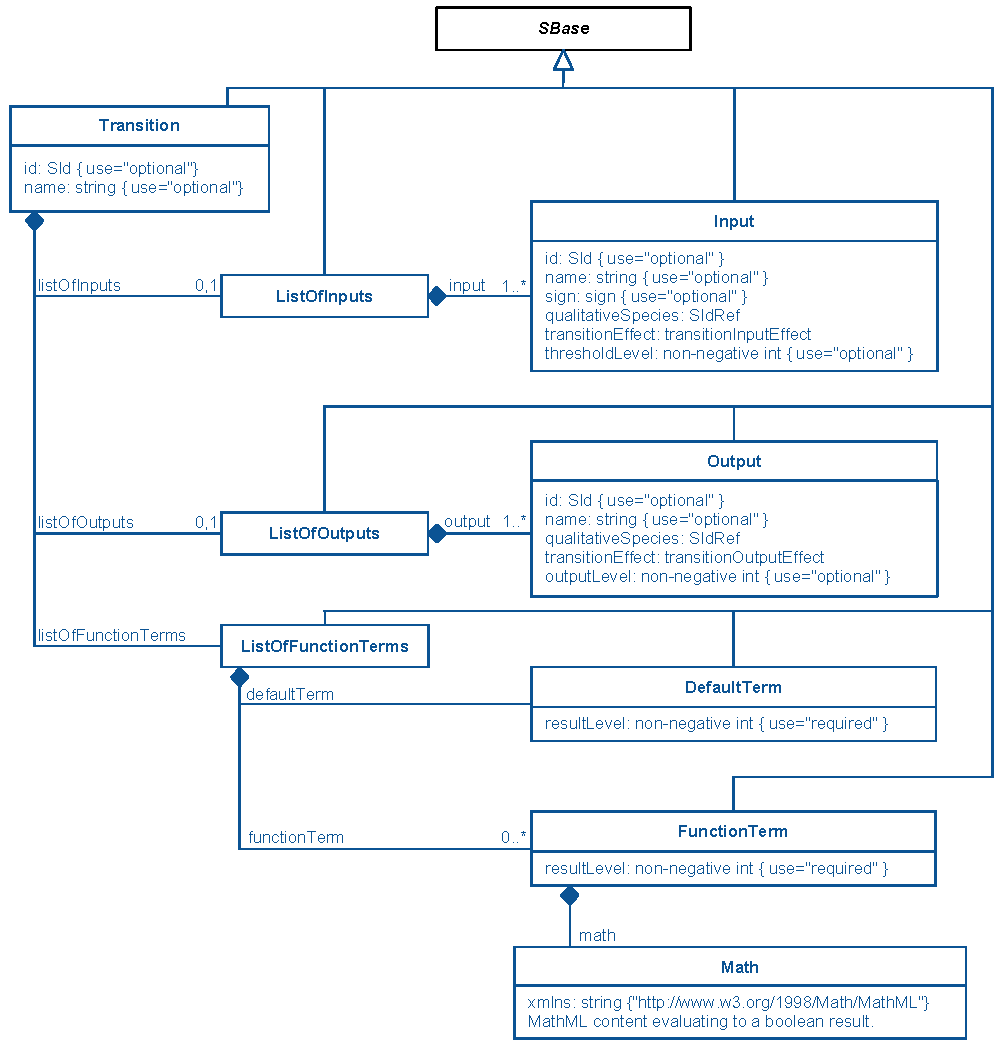
\includegraphics{figs/qual-transition-uml.pdf}
  \caption{The definitions of \Transition, \Input, \Output, \DefaultTerm and \FunctionTerm classes. Note that the \DefaultTerm class is not derived from SBase. }
  \label{qual-transition-uml}
\end{figure}


A \Transition defines the changes in \emph{level} associated with the \QualitativeSpecies  that occur when a \Transition is enabled.  


\pagebreak


In logical models a \Transition is used to specify the logical rule associated with a \QualitativeSpecies (that appears as an \Output of this \Transition). For example, the rule \textit{if} $A > 1: B = 2$ would be encapsulated as a \Transition with \QualitativeSpecies \val{A} as an \Input and \val{B} as an \Output; the \textit{if} $A > 1$ rule being encode by the \token{math} element of a \FunctionTerm with the \token{resultLevel} attribute having a value \val{2}. 


In Petri net models a \Transition is interpreted, using the common Petri net semantics, as events that might occur within the system causing tokens to be moved. The example  in \sec{sub:ex_pn} illustrates a simple Petri net model with two input places, two output places and one transition.



\paragraph{The \token{id} attribute}
A \Transition element has an optional \token{id} attribute of type \primtype{SId}.  In constrast to most SBML classes the \token{id} attribute on a \Transition has no mathematical interpretation.

\paragraph{The \token{name} attribute}
There is an optional \token{name} attribute of type \primtype{string} that should be used
in the same manner as on SBML Level~3 Core
objects; see Section~3.3.2 of the SBML Level~3 Version~1 Core
specification for more information.

%\paragraph{The \token{temporisationType} attribute}
%A \Transition has an attribute \token{temporisationType} of type \primtype{temporisationType} used to indicate the updating policy associated with this \Transition element. This attribute is optional. \tab{transition-temporisation} describes the different updating policies.
%
%\begin{table}[thb]
%  \begin{edtable}{tabular}{p{1in}p{5in}}
%    \toprule
%    \textbf{TemporisationType} & \textbf{Interpretation} \\
%    \midrule
%    \const{timer} & TBD \\
%    \const{priority} & TBD \\
%    \const{sustain} & TBD \\
%    \const{proportion} & TBD \\
%    \const{rate} & TBD \\
%    \bottomrule
%  \end{edtable}
%  \caption{Interpretation of the \token{temporisationType} attribute on a \Transition.} 
%  \label{transition-temporisation}
%\end{table}
%
%\TODO{need more explanation of this}

\subsubsection{The \class{Input} class}
\label{input-class}
The \ListOfInputs contains at least one element of type \Input. 
%A transition with zero inputs can be useful for defining an initial assignment, where the state of an output %depends on a function but not on any input values. An empty list is allowed, and useful for e.g. adding %annotations.
Each \Input refers to a \QualitativeSpecies that participates in the corresponding \Transition.
In Petri nets, these are the input places of the transition. In logical models, they are the regulators of the species whose behaviour is defined by the transition.

\paragraph{The \token{id} attribute}
An \Input element has an optional \token{id} attribute of type \primtype{SId}. The identifier of an \Input can be used as a 
<ci> element within 
math elements included by elements defined within the namespace of the Qualitative Models specification i.e. the \token{math} element of a \FunctionTerm, in which case it it interpreted as the \token{thresholdLevel} of this \Input. Note that for SBML Level~3 Version~1 identifiers from a given package cannot be referenced by elements outside that package. 

\paragraph{The \token{name} attribute}
There is an optional \token{name} attribute of type \primtype{string} that should be used
in the same manner as on SBML Level~3 Core
objects; see Section~3.3.2 of the SBML Level~3 Version~1 Core
specification for more information.


\paragraph{The \token{qualitativeSpecies} attribute}
The required attribute \token{qualitativeSpecies}, of type \primtype{SIdRef}, is used to identify the \QualitativeSpecies that is the \emph{input} of this \Transition.  The attribute's value must be the identifier of an existing \QualitativeSpecies object in the model.  This attribute is comparable with the \token{species} attribute on the \sbml{SpeciesReference} element.

\paragraph{The \token{thresholdLevel}  attribute}
The \token{thresholdLevel} is a non-negative \primtype{integer} that can be used to set the threshold level of the particular input. This attribute relates to the contribution of this input required for the transition to take place. In logical regulatory models, it refers to the threshold level that must be reached or exceeded in order for the regulation to take place, while in a Petri net, it refers to the number of tokens required to enable the transition (weight of the arc connecting the input place to the transition). Whether the \emph{level} of a \QualitativeSpecies should reach or exceed the \token{thresholdLevel} in order for the \Transition to occur will be encoded in the \token{math} elements of the FunctionTerms listed for the given \Transition.

The \token{thresholdLevel} is used by the FunctionTerms associated with the containing \Transition to determine the applicable \token{resultLevel} that should be applied. The \token{id} of the \Input represents this value and can be used in the \token{math} element of a \FunctionTerm. When defined, this attribute should be coherent with the content of the \FunctionTerm, {\em i.e.} if a \emph{number} is used in the \FunctionTerm to compare the current \emph{level} of a species, this number must correspond to the \token{thresholdLevel} of the corresponding \Input. Since a \emph{number} can be used within the \FunctionTerm to represent the \token{thresholdlevel} of an \Input it is not compulsory to use this attribute to specify the value. A missing \token{thresholdLevel} attribute merely implies that the threshold is incorporated into the \FunctionTerm using a number.

\paragraph{The \token{transitionEffect} attribute}
Each \Input has a required attribute \token{transitionEffect} of type \primtype{transitionInputEffect} which describes how the \QualitativeSpecies referenced by the \Input is affected by the \Transition. \tab{transition-input} shows the possible values with the interpretation of each value.


\begin{table}[thb]
  \begin{edtable}{tabular}{p{1in}p{5in}}
    \toprule
    \textbf{TransitionInputEffect} & \textbf{Interpretation} \\
    \midrule
    \const{none} & The level associated with the \token{qualitativeSpecies} is not modified.\\
    \const{consumption} & The level of the \token{qualitativeSpecies} is decreased by the \token{resultLevel} of the applicable \FunctionTerm possibly modified by the \token{thresholdLevel} of the \Input.\\
    \bottomrule
  \end{edtable}
  \caption{Interpretation of the \token{transitionEffect} attribute on an \Input.
Note: as discussed in \sec{loft-class} the 'applicable \FunctionTerm' refers to whichever \FunctionTerm in the \ListOfFunctionTerms evalutaes to \val{true} or the \DefaultTerm if all of the \FunctionTerm objects evaluate to \val{false}.} 
  \label{transition-input}
\end{table}

The following example illustrates the interpretation of the transitionEffect attribute. 

\begin{example}
<listOfInputs>
    <input qualitativeSpecies="A"   transitionEffect="none"        thresholdLevel="2" />
    <input qualitativeSpecies="B"   transitionEffect="consumption"/>
    <input qualitativeSpecies="C"   transitionEffect="consumption" thresholdLevel="2" />
</listOfInputs>
\end{example}

In the case of qualitativeSpecies \val{A} the \token{level} is unaltered by the \Transition and hence the \token{transitionEffect} attribute is set to \val{none}. 

The \token{level} of qualitativeSpecies \val{B} is reduced; hence the \token{transitionEffect} is \val{consumption}. The \token{level} is reduced by the value of the \token{resultLevel} from whichever \FunctionTerm is applicable  (see \ref{sec:function-term}). 

Similarly, the \token{level} of \val{C} is also reduced, but on this occasion by $2$ (the \token{threholdLevel}) times the \token{resultLevel} of whichever \FunctionTerm is applicable. 

It should be noted that in logical models the \token{transitionEffect} is always set to \val{none}, while in Petri nets, it can be set to \val{none} (indicating a read arc) or to \val{consumption}.  The Petri net example in \ref{examples} provides a further example of the use of the \token{transitionEffect} and \token{thresholdLevel} attributes. 

%\TODO{An example of a resultLevel modified by a thresholdLevel}

 
\paragraph{The \token{sign} attribute}
The \token{sign} of type \primtype{sign} can be used as an indication as to whether the contribution of this input is positive, negative, both (dual) or unknown. This enables a model to distinguish between stimulation and inhibition and can facilitate interpretation of the model without the mathematics. The sign is particularly used for visualization purposes and has no impact on the mathematical interpretation. This attribute is optional.


\subsubsection{The \class{Output} class}
\label{output-class}

The \ListOfOutputs contains at least one element of type \Output. 
%A transition with zero outputs can be useful for modelling the effect of the environment. For example, in %Petri nets, a sink transition (with no output) will consume all tokens arriving in its input places; in logical %models, there should not be such transitions. 

Each \Output refers to a \QualitativeSpecies that participates in (is affected by) the corresponding \Transition.  In Petri net models these are the output places of the transition.  

\pagebreak
In a logical model, a \QualitativeSpecies should be referenced in at most one \ListOfOutputs, (that of the \Transition defining the evolution of this species). This restriction is discussed in more detail in \ref{best-practices}. When a \Transition has several outputs, it is because the referenced species share the same regulators and the same logical rules.




\paragraph{The \token{id} attribute}
An \Output element has an optional \token{id} attribute of type \primtype{SId}.  The identifier of an \Output can be used as a 
<ci> element within 
math elements included by elements defined within the namespace of the Qualitative Models specification i.e. the \token{math} element of a \FunctionTerm, in which case it it interpreted as the \token{outputLevel} of this \Output. Note that for SBML Level~3 Version~1 identifiers from a given package cannot be referenced by elements outside that package. 

\paragraph{The \token{name} attribute}
There is an optional \token{name} attribute of type \primtype{string} that should be used
in the same manner as on SBML Level~3 Core
objects; see Section~3.3.2 of the SBML Level~3 Version~1 Core
specification for more information.



\paragraph{The \token{qualitativeSpecies} attribute}
The required attribute \token{qualitativeSpecies}, of type \primtype{SIdRef}, is used to identify the \QualitativeSpecies that is the \emph{output} of this \Transition.  The attribute's value must be the identifier of an existing \QualitativeSpecies object in the model.  This attribute is comparable with the \token{species} attribute on the \sbml{SpeciesReference} element.

\paragraph{The \token{outputLevel} attribute}
The \token{outputLevel} is a non-negative \primtype{integer} used along with the \token{transitionEffect} to specify the effect of the \Transition on the corresponding \QualitativeSpecies. It does not specify the result of a \Transition; this is done by using the \token{resultLevel} attribute on a \FunctionTerm. However, in Petri nets, it relates to the weight of the arc connecting the transition to the output place and may be multiplied by the \token{resultLevel} in a \val{production} situation. In logical models there is no interpretation of the \token{outputLevel} attribute as the outcome of a \Transition is always an assignment to the \token{resultLevel} defined by the \FunctionTerm. 

The \token{outputLevel} attribute is optional since if the \token{transitionEffect} is set to \val{assignmentLevel} (as in logical models), it has no meaning. However, where the \token{transitionEffect} of the \Output is set to \val{production} (as in Petri net models) the resulting level of the \QualitativeSpecies is the \token{resultLevel} from the appropriate \FunctionTerm multiplied by the \token{outputLevel}. Since there are no default values in SBML Level~3, when the \token{transitionEffect} is set to \val{production} the \token{outputLevel} attribute must have a value.

\paragraph{The \token{transitionEffect} attribute}
Each \Output has a required attribute \token{transitionEffect} of type \primtype{transitionOutputEffect} which describes how the \QualitativeSpecies referenced by the \Output is affected by the \Transition. \tab{transition-output} shows the possible values with the interpretation of each value.



\begin{table}[thb]
  \begin{edtable}{tabular}{p{1in}p{5in}}
    \toprule
    \textbf{TransitionOutputEffect} & \textbf{Interpretation} \\
    \midrule
    \const{production} & The level of the \token{qualitativeSpecies} is increased by the \token{resultLevel} of the applicable \FunctionTerm possibly modified by the \token{outputLevel} of the \Output.\\
    \const{assignmentLevel} & The level of the \token{qualitativeSpecies} is set to the \token{resultLevel} of the selected term. \\
%    \const{assignmentSymbol} & The symbol of the \token{qualitativeSpecies} is set to the \token{resultSymbol} of the selected term.\\
    \bottomrule
  \end{edtable}
  \caption{Interpretation of the \token{transitionEffect} attribute on an \Output. 
Note: as discussed in \sec{loft-class} the 'applicable \FunctionTerm' refers to whichever \FunctionTerm in the \ListOfFunctionTerms evalutaes to \val{true} or the \DefaultTerm if all of the \FunctionTerm objects evaluate to \val{false}.} 
  \label{transition-output}
\end{table}
\pagebreak
The following example illustrates the interpretation of the transitionEffect attribute. In the case of qualitativeSpecies \val{A} the \token{level} is assigned the \token{resultLevel} from the whichever \FunctionTerm is applicable, whereas the \token{level} of qualitativeSpecies \val{B} is increased by \token{resultLevel} (effectively \token{resultLevel} times $1$ (\token{outputlevel})). Similarly, the \token{level} of \val{C} is increased by $2$ (\token{outputlevel}) times \token{resultLevel} (see also Petri net example in \ref{examples}). 

\begin{example}
<listOfOutputs>
    <output qualitativeSpecies="A"   transitionEffect="assignmentLevel"/>
    <output qualitativeSpecies="B"   transitionEffect="production"  outputLevel="1"/>
    <output qualitativeSpecies="C"   transitionEffect="production"  outputLevel="2" />
</listOfInputs>
\end{example}

In logical models the \token{transitionEffect} is set to \val{assignmentLevel} whilst in standard Petri nets it is set to \val{production}.  It is envisioned that to encode High Level Petri nets it will be necessary to allow the use of \\* \val{assignmentLevel} as an \Output \token{transitionEffect}; however considering the implications of this is left to future versions of the specification (see \sec{apdx:apdx-future}).

\subsubsection{The ListOfFunctionTerms class}
\label{loft-class}

The \ListOfFunctionTerms may contain any number of \FunctionTerm elements, and must contain exactly one \DefaultTerm.  Each \FunctionTerm encodes the conditions under which this term is selected.  The \DefaultTerm describes the result of the \Transition applied by default ({\em i.e.} when no term evaluates to \val{true}). 
\bigskip
\subsubsection{The DefaultTerm class}
\label{defaultTerm-class}
The \DefaultTerm defines the default result of a \Transition.  This term is used if there are no other \FunctionTerm elements or if none of the \sbml{Math} elements of the \FunctionTerm elements evaluates to \val{true}. 

\paragraph{The \token{resultLevel} attribute}
The default result is described by a \token{resultLevel}. This attribute is required.

The \token{resultLevel} is a non-negative \primtype{integer} describing a level.  The \token{resultLevel} is used; possibly together with the \token{thresholdLevel} or \token{outputLevel} to determine the level of a \QualitativeSpecies resulting from the \Transition. 
\bigskip
\subsubsection{The \class{FunctionTerm} class}
\label{sec:function-term}

Each \FunctionTerm is also associated with a result  and in addition to a Boolean function inside a \sbml{Math} element that can be used to set the conditions under which this term is selected.

\paragraph{The \token{resultLevel} attribute}
The result of the term is described by a the required attribute \token{resultLevel}.

The \token{resultLevel} is a non-negative \primtype{integer} describing a level.   The \token{resultLevel} is used; possibly together with the \token{thresholdLevel} or \token{outputLevel} to determine the level of a \QualitativeSpecies resulting from the \Transition. 

\paragraph{The \sbml{Math} element}
Each \qual{FunctionTerm} holds a \primtype{boolean} function encoded in a \sbml{Math} element, using the subset of MathML 2.0 as defined in SBML L3v1 Section 3.4.6. Since the concept of \emph{time} is beyond the scope of this specification it is recommended that the \token{csymbols} \val{time} and \val{delay} that explicitly involve \emph{time} are not used.

This element encodes the conditions under which the \FunctionTerm is selected. When the \sbml{Math} element contains the identifier of a \QualitativeSpecies, \Input or \Output, this identifier represents the \emph{level}, \token{thresholdLevel} or \token{outputLevel} of the corresponding element. It should be noted that for the purposes of this specification these all have integer values. Tools working with Boolean  models with allowed levels restricted to \val{0} and \val{1} may choose to interpret the identifiers as \primtype{boolean}.  However this specification  requires that any \token{math} element unambiguously returns a \primtype{boolean} function. Thus, assuming A is an identifier representing a \emph{level}, the math expression \textit{if} $(A)$ is not valid and must be explicitly written as \textit{if} $(A == 1)$ (or similar). Tools may need to consider this when exporting models.

\subsubsection{Mathematical interpretation of Transitions and FunctionTerms}
\label{math-interpret}

In the Qualitative Models  package, {\em transitions} are the central mechanism for describing processes that change the levels of the qualitative species of the model. Here, we clarify their interpretation in the framework of logical modelling.

The {\em function terms}  of a \Transition define the transition function for one \qual{QualitativeSpecies}, {\em i.e.} its state transitions depend on the levels of the species that appear as input of that transition (its "regulators"). The {\em function terms} together with the {\em default term} thus define a state transition table indicating what level the qualitative species will move to (target level), based on the current level of its regulators. In the case of multi-valued \emph{levels} (as opposed to Boolean), this evolution proceeds step-wise towards the target level, {\em i.e.} each component of two successor states of the system differ at most by $1$. The \qual{QualitativeSpecies} affected by the \Transition is referenced by the \Output element. In the situation where there is more than one \Output listed, the referenced species share the same regulators and the same logical rules.

The model must be fully defined. Whatever the state of the system, one single value must apply (that of the \DefaultTerm or the \token{resultLevel} of a \FunctionTerm). More than one \FunctionTerm can share the same \token{resultLevel}, which is the equivalent to a single term holding the {\bf disjunction} (OR) of all these terms.  There must be no conflicting terms:  whenever multiple function terms apply (are true), their \token{resultLevel} must be the same. 

It should be noted that the \emph{level} associated with a \qual{QualitativeSpecies} has values from 0 up to the \token{maxLevel} (where declared). The mathematics of the model (i.e. the \FunctionTerm and \DefaultTerm element together with the \token{transitionEffect}) should not allow the \emph{level} to either become negative or exceed the maximum.

Importantly, given a model, one has then to choose an updating policy that defines how enabled transitions are processed (synchronously, asynchronously, etc.). However, this information is not part of the model {\em per se}. 


\subsection{Namespace scoping rules for identifiers}
\label{sec:ns-id}

The values of any \token{id} attribute  of type \primtype{SId} within the qual namespace are considered to have the same scope as any \token{id} attribute with type \primtype{SId} in the core SBML namespace. Thus the values of the attributes
  \token{id} and \token{qual:\-id} must be unique across the set of all \token{id} and
  \token{qual:\-id} attribute values of all objects in a model. In addition to those classes of objects specifed in the SBML Level 3 Version 1 Core specification;
  \Model, \FunctionDefinition, \Compartment,
  \Species, \Reaction, \SpeciesReference, \ModifierSpeciesReference,
  \Event, and \Parameter objects, this includes the following objects from this Qualitative Modelling package: \qual{QualitativeSpecies}, \Transition, 
  \Input and \Output.
